\chapter{Introduction}

Cities are a central feature of human society - Human beings are increasingly an urban species. Cities are one of the primary sources of technological development and increasing wealth. Behind these observations is a fundamental feature demonstrated in the recent literature on scaling laws: the productivity of cities increases super-linearly in population. Cities are the locus of a positive feedback loop: rising populations raises productivity, rising productivity attracts more people and resource.

Cities are where people live and work, where a great deal of production is concentrated, in addition to being where wealth is created and accumulated, cities are also where income is actually distributed. 

In Canada, there is a housing crisis. In the last few years, the need for affordable housing has come into focus as one of the most pressing issues facing Canadians. As more and more Canadians are finding housing unaffordable, the effects are being seen in everything from declining home ownership rates to an increasing number of Canadians unable to afford housing at all.

There has been extensive work on the drivers of the crisis, including supply shortages, stagnating incomes, and the finacialization of housing ownership.

There's been less work on the implications for productivity. The housing crisis raises the question of whether Canadian cities can continue to attract people and accumulate wealth for its residents and industries, whether in fact it can even sustain their growth.

This thesis presents a spatial model of the city that incorporates distributional issues and financialization and allows us to examine the productivity implications of the housing crisis. The model that incorporates the scaling of productivity in cities within a standard urban model. 
The urban model is based on those developed in geography, planning and urban economics. The organizing principle in  the spatial models of all three disciplines is an economic variable, land rent, which is the link to distribution, financialization and continuing productivity. *** (another sentence on why this is great)

The analysis makes clear that in addition to the recognized distributional consequences, the housing crisis has productivity impacts that should be considered in developing urban and housing policy. 


\subsection{OVERVIEW OF DOCUMENT}
\color{blue}

\textbf{In chapter XXX}  we link classical rent theory, neoclassical production theory, neoclassical growth theory, the scaling literature, and urban spatial models.
To show how our model is directly connected with this broad collection of linked theories, we use the Cobb-Douglas function, which is used across this entire range of literature 

After we develop the mathematical description of the relationship among these will discuss  in more detail, rent theory and our contribution, scaling laws, ......  and other issues in the literature that draw on parts of this model and 

???  apply to the specific situation we're in why rent theory is related to discussions of exploitation why it might lead the inefficiencies, whether or not this links with other important models in the literature.

\textbf{In chapter XXX} we  provide a description of finacialization and show it is a a form of rent-seeking in the housing market and ?? the potential consequences of fiancialization in the housing market. 



\textbf{In chapter XXX} we  describe an illustrative agent-based model of the urban system. Most of the analysis of urban systems has employed analytical models with roots that go back to von Thunen () and more recently Alonzo. These models are extremely useful, but necessarily abstract from the concrete  and variable individual behaviour and  the details  of dynamics that make real cities path-dependent. XXX (Dawn) have shown that agent-based models can reproduce the features of the analytical models, at least in simple cases. 

ABMs can be run multiple times to produce distributions of expected outocomes, which makes them valuable in planning exercises. They also do not require  that we use a representative agent to make them tractable. Our model is intended to be elaborated  for such use. 

After we develop the mathematical description of the relationship among these will discuss in more detail, various relevant applications, and issues in the literature that draw on parts of this model and apply to the specific situation we're in why rent theory is related to discussions of exploitation why it might lead the inefficiencies, whether or not this links with other important models in the literature.


\color{red}
Because we draw on a wide range of methods and literatures, we discuss the relevant literature and  nethodologies in the chapters where they apply 

\color{black}


Methodological questions: 

    - agent models (integrating theory more completely into agent models)
    
    - rent theory

Core model

    - static version
    
    - dynamic version

Simulations

Result---> hysterisis

policy

\subsubsection{OR (rougher):}

1. the core model and analysis - do a model of the endogenous dynamics of the model.

2. the resilience analysis -
but this is coupled with a larger system. we're interested in how it is coupled..

low interest rates have been key to financialization 
now they're going up?

we drive the system with signals to see how. and look at the external driving variables.

but what happens with changing interest rates? to explore we drive the system with external signal to explore how it is coupled with the larger economy and get an interesting resilience result, that it is actually a kind of ratchet pumping wealth out of communities on the upswing and on the downswing.

add interest, get a result which is hysteresis, which has policy implications
We get predictions about the implications of rising interest rates.

3.  policy analysis - finally we take a second step out to position the model within a larger dynamical system and do a systems analysis of the model and suggest policy implications. 

----------

% ?Ideally, an analysis of the current state of cities will incorporate supply, 
what do we want for the long introduction and background

\textbf{Ricardo concluded, significantly, that, ``It follows then, that the interest of the landlord is always opposed to the interest of every other class in the community.'' }


Our model has three stages: first, a production function, modeling how urban regions generate wealth,  second a spatial model of an urban housing market, and third, an analysis of distribution within that model 

In this section, we introduce the basic structure of the production side and connect it to the literature on urban scaling. The basic scaling result at the level of the city allows us to incorporate the effect of agglomeration in a standard  circular-city model in a simple way, avoiding the need to explicitly model labour markets and firms.\footnote{Explicitly modeling labour markets and firms is a natural way to specify the model more completely, but it would require introducing many ancillary assumptions and selecting among alternative models of agglomeration, when when we want to focus on distributional and growth-affecting features of the system.}

\begin{enumerate}
    \item to introduce  the productive nature of cities we basically assume the presence of scaling. Given  that the scaling literature gives us an estimate of the economies of scale in a production function this allows us to simplify the model and focus on the features of the urban system rather than on fully specifying a production system. In our model, the city  exhibits economies of scale with respect to population directly. 

     \item  productivity of the city to generates an economic value for land that gives rise to rents

    \item  the rental value of land structures the spatial structure of the city

    \item we exploit the rent model and transport costs to get  distributional consequences
\end{enumerate}

\color{red}
\chapter{Antecedents of modern Urban Rent theory}
In this chapter, we link classical rent theory, neoclassical production theory, neoclassical growth theory, the scaling literature,  and urban spatial models. 

We use the Cobb-Douglas function %, which is used to cross this entire range of literature 
to illustrate each link and to show how our  model is directly connected with this broad collection of linked theories. Our model connects to the results in this chapter at four points:



\section{Classical production and distribution theory}


 \subsection{Ricardo}

Modern neoclassical production theory can be seen as having one of its origins in  Classical economic theory going back to the Physiocrates. The physiocratic school of economics was the first to see labor as the sole source of value but, for the physiocrats, in the context of the prevalent European rural society of the time, only agricultural labor created a surplus. Ricardo's famous 1815 discussion of capital and  land rent \footnote{ %\href{http://la.utexas.edu/users/hcleaver/368/368RicardoOnCornLaws.html}{An Essay on the Influence of a low Price of Corn on the Profits of Stock}; 
showing the Inexpediency of Restrictions on Importation: With Remarks on Mr Malthus' Two Last Publications: "An Inquiry into the Nature and Progress of Rent," and "The Grounds of an Opinion on the Policy of restricting the Importation of Foreign Corn" } 
provides the canonical reference. He considers three-factor, three-class model with great precision but without the use of mathematics.   

In Ricardo's analysis and in classical economics in general, the income or landowners, land rent, is a surplus value\footnote{``By rent I always mean the remuneration given to the landlord for the use of the original power of the land.'' David Ricardo corn laws note 7.}. 
and as Saunders pointed out in 1902, ``Of the concrete forms of income that have usually been classed as surplus, the rent of land was the earliest to be defined; and so prominent a position has been given to it that the terms " rent" and " surplus" have come to be used interchangeably.''\footnote{Rent in Modern Economic Theory: An Essay in Distribution Author(s): Alvin Saunders Johnson, Publications of the American Economic Association, Nov., 1902, 3rd Series, Vol. 3, No. 4 (Nov., 1902), pp. 1-129}. 

The great social question that Ricardo addressed  was who gets the surplus. % The question was pressing because it appeared that landlords were capturing the surplus without contributing to production while many of those who worked that land were very poor. 
We begin with Ricardo and the classical economists because our focus is land rents, but in the context of an urban economy. According to Simon N. Patten, \footnote{Simon N. Patten,  The Quarterly Journal of Economics, volume 7, Issue 3, April 1893, Pages 322–352, https://doi.org/10.2307/1884006 }  Ricardo was ``the first writer to take the industrial phenomenon of city life and to create an economy based upon those characteristics.'' %Ricardo uses his model to explain the distribution of the product of the earth among the “three classes of the community” which is to say, to the owners of land, labour, and capital. 
In a passage that can be seen as a direct precursor to our analysis of urban land rent, Ricardo  wrote in his 1817 Principles of Political Economy, %

\begin{quotation}   
 “The produce of the earth - all that is derived from its surface by the united application of labour, machinery, and capital, is divided among three classes of the community; namely, the proprietor of the land, the owner of the stock or capital necessary for its cultivation, and the labourers by whose industry it is cultivated. ...  But in different stages of society, the proportions of the whole produce of the earth which will be allotted to each of these classes, under the names of rent, profit, and wages, will be essentially different; ”  Chapter 1
\end{quotation}

Land rent is easily illustrated. Imagine a carter who picks up vegetables at the farm gate and transports them into tow, where he sells them to a  storekeeper. He pays  the farmer at one end of the trip and is paid at the other. For simplicity. let's say all farmers have the same cost of production and the carters simply pay that amount at the farm gate and always is paid the merchant price in town. 

Clearly, the carter makes a `profit'  on his trip to the  farm nearest to town, but there is a farm so far out  that transport costs   eat up all the profit on the trip. That is as far as the carter will go. Ricardo termed this the `extensive margin'. 

 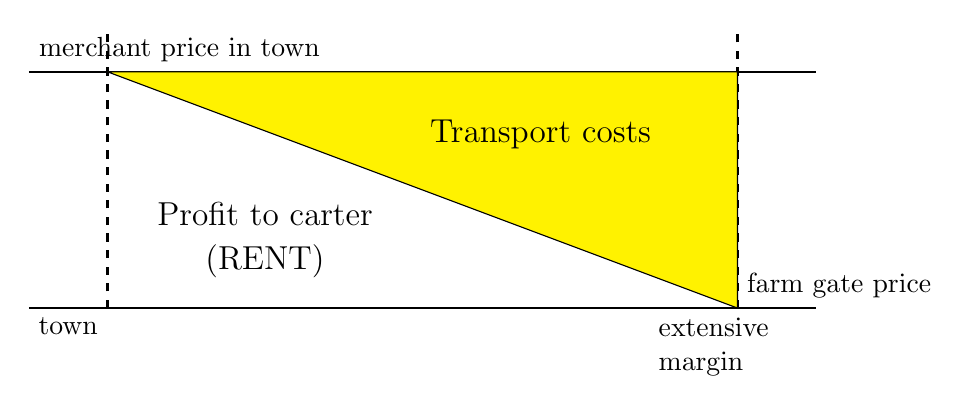
\begin{tikzpicture}[domain=0:2]
%\draw[thick,color=gray,step=.5cm, dashed] (-0.5,-.5) grid (3,3);
%\draw[line width=.01, green ] (0,0) -- (10,0) node[right  ] {Distance};
\node at (1,0) [below left] {town};
\draw[thick ] (0,3)node[above right] {merchant price in town} -- (10,3) ;
\draw[thick ] (0,0)  -- (10,0); 

draw[thick,color=red] (1.5,0) -- (1.5,1) node[below right] {Fixed cost} -- (1.5,1.5) --(10,3.25)node[above left] {total cost};
\draw[thick, dashed ] (1,0) -- (1,3.5) ;
\draw[thick, dashed ] (9,0)node[below,text width=2cm] {extensive margin} -- (9,3.5) ;
%\draw[ultra thick, blue,<-> ] (3,1.8) -- (3,2.5)node[left] {annual rent at a} -- (3,3) ; 
\draw[fill=yellow] (1,3) --(9,3)--(9,0) --cycle;
\node at (9,0)[above right] {farm gate price};
\node  at (6.5,2.2){\large Transport costs};
\node  at (3.,1.2){\large Profit to carter};
\node  at (3.,.6){\large (RENT)};
\end{tikzpicture}   

In the figure, total transport costs are shown as the yellow area. The area below the yellow triangle is profit for  the carter.\footnote{Compare the figure to one developed to illustrate Alonzo's urban model:


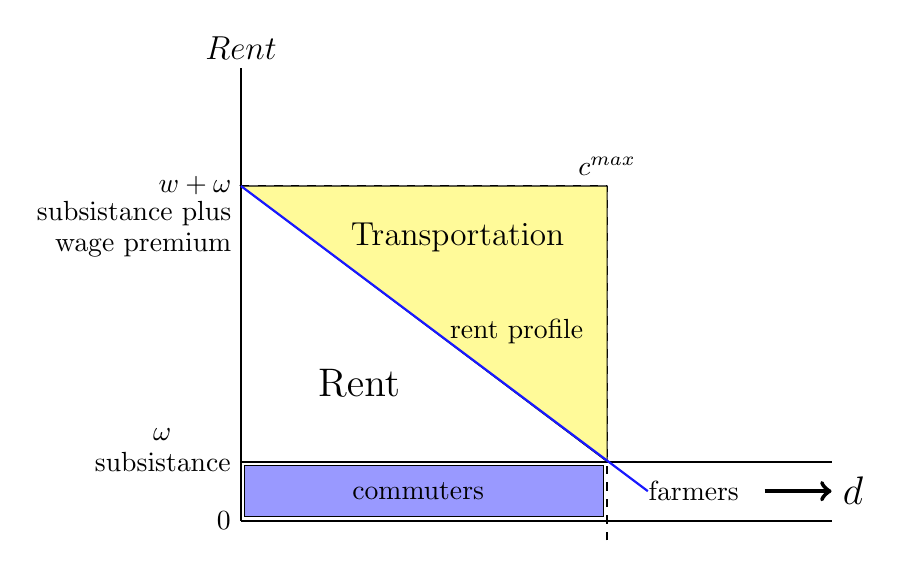
\begin{tikzpicture}[scale=.5]
\def\bndmax{5}        
\def\bndmin{0.2}
\def \n {10}  % height of y axis
\def \d {15}  % length  of x axis
\def \t {.75}  %  cost of transportation per unit x
\def \th {1}   %
\def \w {7}    %  wage premium
\def \om{1.5}%  omega =rural wage Zero for urban population
\def \azero{2}
\def \aprime {-.0}	
\tikzset{func/.style={thick,color=blue!90}}	

\draw [thick] (0,-\om) --(\d,-\om);  			% Zero for rural population
\draw [thick] (0,-\om)node[left]{$0$} --(0,\n);	% Y axis
\node at (0,\n+0.5){\large$Rent$};

\draw [thick] (0,0)node[left]{subsistance}--(\d,0);
\node a t(-2,.7) {$\omega$};
\node[left] at (0,\w){$w+\omega$};
\node[left] at (0,\w-.7){subsistance plus};
\node[left] at (0,\w-1.5){wage premium};	
\draw [dashed, thick](9.3,-2)-- (9.3,\w)node[above]{$c^{max}$};
\draw [dashed, thick](0,\w)-- (9.3,\w);
% solid color for commuters
\draw[fill=blue!40] (0.1,-0.1) rectangle (9.2,-\om+.1);
\draw[fill=yellow!40] (9.30,7.) -- (0,7)--(9.30,0.)--cycle;% Rent \w-.2
\draw[func,domain=0:\w/\t+1] plot [samples=200] (\x,{\w-\t*\x});
\node at (5.5,5.7){\large Transportation};
\node at (7,3.3){rent profile};		%Rent Profile	
\node at (3.,2){\Large Rent}; 		%Rent 
\node at (4.5,-\om/2){commuters};
\node at (11.5,-\om/2){farmers};
\draw [ ultra thick, ->](13.3,-\om/2)--(15, -\om/2)node [right] {\Large $d$};
 
 \end{tikzpicture}


} Together these areas represent the ``produce of the earth'', but only the lower triangle is net income\footnote{ Termed the `\textit{produit net}' by the Physiocrats}.   In modern supply and demand analysis it would be recognized as `producer surplus'.

Now consider Ricardo's case: the land owner delivers the grain to market and receives the merchant price. The profit now accrues to the landowner, and we call it land rent. For Ricardo, it was obvious that the land-owning class captured the land rent.\footnote{In the modern economy, agricultural land rents may be captured by corporations,  either by owning the land or by controlling the supply chain.}  Landlord income is a locational land rent that exists  because of the land's proximity to the market. 

Notice how the land rent declines with distance from the town,\footnote{It also declines as we move onto less fertile land.} At the extensive margin the land rent falls to zero. Even fertile land beyond the extensive margin will not be farmed because the product cannot be transported to market at a profit.\footnote{This simple example assumes that the land is uniformly productive and that there is only one product that can be marketed. Johann Heinrich von Th\"unen, in The Isolated state (Der isolierte Staat (1826)), provide a more complex analysis based on the same principles.} Transportation costs and the price of produce in town determine the size of the  rent triangle and therefore the amount of rent captured by the land-owning class.\footnote{The debate about the  `Corn Laws" that Ricardo  was engaged in was about whether Britain would allow wheat form Canada and Australia to enter, reducing the price of wheat and therefore reducing the income and influence of the land-owning class.} 


%\subsection{A more explicit treatment}
Ricardo expounded a theory of land rent, but he did not write down a formal production function as later neoclassical theorists would. In modern notation, Ricardo's model can be written


\begin{equation} 
Y=F(K,L,N).
\label{Eqn:Prod1}
\end{equation} 
where $K$ is capital, $L$ is labour and $N$  is the natural resource  land.\footnote{In principle any number of factors can be included.} 
Ricardo does not specify a functional form, but, like mathematical neoclassical economists, he does assume diminishing returns to all factors. The landlord  receives the surplus generated by the land and the rest of the value of production goes to labour and to any capital employed in improving the land. 

The value of the land is the present discounted value of the surplus it generates.

Most modern neoclassical treatments of production simplify by omitting land: 

\begin{equation} 
Y=F(K,L).
\label{Eqn:Prod1}
\end{equation} 

Leaving land out of the model makes sense for a variety of reasons. According to the Ricardian theory, rent is a surplus above cost. It does not, therefore enter into price. Land is a fixed factor for society as a whole that is not consumed in  the process of production.  Furthermore, neoclassical treatments of production focus price determination based on the cost of the last unit used, the marginal  unit of input, while rents are generated on all of the inframarginal units, those units used earlier, which are more productive. The marginal unit of land generates no rents. In neoclassical analysis, the rents disappeared from view for this reason. This difference is at the heart of the distinction between classical and neoclassical economic theory. 

Classical rent re-appears in neoclassical theory as `economic rent' ``a money payment made for a factor of production that is over and above the minimum payment to keep it in its present use,''  as quasi-or pseudo-rents (non-equilibrium rents that will be competed away in a competitive equilibrium according to Marshall.\footnote{see Lewis Cecil Gray Rent Under the Assumption of Exhaustibility, Quarterly Journal of Economics, May, 1914, Vol. 28, No. 3 (May, 1914), pp. 466-489}),  as consumer  and producer surplus in supply and demand analysis,  as rent profiles or Pseudo-rent curves in urban theory, as a major concern on resource economics, and the theory of rent-seeking. Economic rent is a surplus insofar as its payment is not necessary to ensure a supply of a particular factor of production. 


% HOUSING RENT IN THE NATIONAL ACCOUNTS
%   Owner-occupied housing is included in Peersonal Consumption Expenditure because the National Income and Producgt Accounts (NIPAs) treat the owner-occupant as if it were a rental business, or in other words, a landlord renting to him or herself. That is, BEA imputes a value for the services of owner-occupied housing (space rent) based on the rents charged for similar tenant-occupied housing, and this value is included in GDP as part of personal consumption expenditures. This imputation is necessary in order for GDP to be invariant when housing units shift between tenant occupancy and owner occupancy.


%Ricardo  clearly understood and used the concept of diminishing marginal product. This shows in his use of the terms ``extensive margin'' and ``intensive margin'' to explain the income of the landowner. He focussed on the difference between the cost of production on a unit of land and the revenue generated. The landlord would rent out all the land which generated at least enough to pay all the costs. Anything in excess of the costs could be charged as land rent to a tenant farmer.



%Clearly in his model there are two basic productive factors, land and labour. The landlord  receives the surplus generated by the land and the rest of the value of production goes to labour. 
Recent urban models, on the other hand, tend to ignore the production process and consider the locational implications of land and transportation costs location of people. Wealth distribution is often ignored. 

\subsection{Marx}

%Ricardo, agreeing with Malthus, essentially assumes that the wage is  just sufficient to reproduce the labouring class.\footnote{``In the natural advance of society, the wages of labour will have a tendency to fall, as far as they are regulated by supply and demand; for the supply of labourers will continue to increase at the same rate, while the demand for them will increase at a slower rate.''} He then explains the distribution of the fruits of labour on the land among the main classes of the economy.

 Marx shifted attention to the manufacturing economy in which the owners contributed the machinery, buildings, and even working capital to fund the workers until the product can be sold. %This contribution must be accumulated from their profits in the preceding cycle of production,  and has to be reinvested once the revenues of the current round have come in and the bills have been paid. Marx actually describes a circuit of capital from its form as money to its form as physical capital. 
As in Ricardo, however, labour is in surplus and capital is scarce. As in Ricardo the scarce factor owned by a special class - now the capitalists, is able to appropriate the is able to capture the surplus value. %Like Ricardo,  Marx saw the appropriation of surplus as without moral justification. 

Marx pointed to a new dynamic in capitalist systems - that productive capital is not fixed as land is, but  expands as surplus is reinvested. He famously suggested that the expansion will eventually outrun the expansion of demand and the rate of return will fall, leaving capitalists unwilling to invest and creating a crisis. 


 
\subsection{Henry George} 
  Henry George, an influential American political economist,\footnote{Progress and Poverty: An Inquiry into the Cause of Industrial Depressions and of Increase of Want with Increase of Wealth: The Remedy (1879) book by social theorist and economist Henry George.}  returned to land rent with a new insight based on the emergence of the capitalist city: ``With the growth of population, land grows in value, and the men who work it must pay more for the privilege.'' For George the owners of urban land extract surplus in exactly the same way that owners of agricultural land in Ricardo's analysis. Where Marx saw  the extravagant productivity of capital  as the source of capitalist crises, George saw the extraction of wealth by land speculators as the mechanism that would bring on crises.
  
  Since land rent is not created by its owners, George argued that land rent should be seen as a social income - that it could be used to pay for all the needs of the community. The clearest statement of this view is found in Progress and Poverty: "We must make land common property." The same view was expressed by the Physiocrats who concluded  that ``ground rents'' should be the source of most or all taxes. They defined ground rent as that portion of all rent which is attributable only to the size and location of the parcel. George's analysis the `single tax' movement, which sought to shift all taxation to land  and resource rents.   
  
  In 1977, Joseph Stiglitz  showed, using a standard urban model, identified the conditions in which Henry George's "single tax" is  the only tax necessary to finance public expenditures.\footnote{Arnott, Richard J.; Joseph E. Stiglitz (November 1979). "Aggregate Land Rents, Expenditure on Public Goods, and Optimal City Size" (PDF). Quarterly Journal of Economics. 93 (4): 471–500. doi:10.2307/1884466. JSTOR 1884466. S2CID 53374401 }   The logic is fairly simple: if the public good increases productivity or the attractiveness of a city, attracting more people or businesses, land rents rise, and investment in the public good should proceed until the marginal cost of the public good is equal to the increase in land rent it brings. The result is now called the `Henry George theorem.'


The classical economists agreed that rents are unearned income. They did not emphasize, as George did, that land rents arise from labour's proximity to urban population and production.\footnote{To be fair, it was not lack of understanding, that the omission reveals, but rather lack of interest in explicitly examining urban land rent from residential or even industrial purposes.}% Ricardo von Thunen, Marx, Cantillon all grasped the notion of proximity to the market as part of the source land rent. The discussions seem to not gone farther than discussions of diffeerential and rents, however.  I just am not aware of them explicitly examining urban land rent for residential or even industrial purposes. 

%The need to be near a market or prodduction center is easily seen by considering a population at the carrying capacity of the land with individuals supporting themselves using purely local resources. There can be no land rent in this case. If a city rises that must be supplied from those still on the land, land close enough to the city will generate land rent. The value of the land is created by proximity to the city.



%  no separate and comprehensive data are provided on the amounts of land rents and subsoil rents charged and earned, because they are not officially regarded as part of value-added, and consequently are not included in the calculation of GDP (except for the value of productive lease contracts)     https://en.wikipedia.org/wiki/Differential_and_absolute_ground_rent#Rent_in_macro-economics    \href{https://en.wikipedia.org/wiki/Differential_and_absolute_ground_rent#Rent_in_macro-economics}{Wikipediat article on differential rent}



  \subsection{John Bates Clark and neoclassical distribution theory}
  Classical theories of distribution showed that ownership of a scarce and non-produced factor, land, was the  basis of rent extraction by the class of landowners. Profits were a bit puzzling in this context - Capital also earns its return from scarcity. Marshall pointed out, however, that scarcity profits (i.e., rent) would normally be competed away  as entrepreneurs entered the market in pursuit of those `excess' profits. He used the term `pseudo-rents' for these unearned but temporary incomes.\footnote{Alvin Saunders Johnson. Rent in Modern Economic Theory: An Essay in Distribution. AEA 3rd Series, Vol. 3, No. 4 (Nov., 1902), pp. 1-129 (129 pages)}

  
 John Bates Clark was one of the pioneers of marginalism and the neoclassical theory of  distribution.  The marginalist approach emphasized the rational decisions of economic agents in allocating their resources would lead them to allocate resources according to the value of the marginal product of the resource in production.  Initially a socialist like George, by 1986 he was praising the dynamical process of competition partly in opposition to the single tax movement George had initiated.  His (1891) ``Distribution as Determined by a Law of Rent,'' argued that, given  competition and homogeneous factors of production labor and capital, the division of the social product will be according to the productivity of the last (or marginal) physical input of units of labor and capital.\footnote{Responding to the "indictment that hangs over society" that it involves "exploiting labor," Clark wrote:

    It is the purpose of this work (his 1899 'Distribution of Wealth) to show that the distribution of the income of society is controlled by a natural law, and that this law, if it worked without friction, would give to every agent of production the amount of wealth which that agent creates. However wages may be adjusted by bargains freely made between individual men (i.e., without labor unions and other "market imperfections", the rates of pay that result from such transactions tend, it is here claimed, to equal that part of the product of industry which is traceable to the labor itself; and however interest (i.e., profit) may be adjusted by similarly free bargaining, it naturally tends to equal the fractional product that is separately traceable to capital.} 
 
Clark's analysis of income distribution does not contradict the classical view of rents, it simply displaces the analysis to the point where a competitive equilibrium prevails, and shifts attention away from the distribution of land rents. Rents are not earned by the marginal unit of land and  

\section{Neoclassical production theory}
The concept of a production function used by increasingly mathematical neoclassical economists and  rapidly developing statistical techniques  naturally led to attempts to identify the precise functional form that would describe the contributions of labour, capital, and income to output.
 
Mathematician Charles Cobb and Economist Paul Douglas came up with a specific and very convenient functional form\footnote{Cobb, C. W.; Douglas, P. H. (1928). "A Theory of Production"  American Economic Review. 18 (Supplement): 139–165. JSTOR 1811556. Retrieved 26 September 2016. The function had apparently previously been used by Knut Wicksell, Philip Wicksteed, and L\'eon Walras.} that captured much of what economists were talking about. The function is just a generalized arithmetic mean:
 
 \[Y=AK^\alpha L^\beta\]
 where $A$ is a constant scale factor, commonly called `Total Factor Productivity. This function becomes the workhorse of neoclassical growth theory in the second half  of the 20th century. Our urban model is a direct heir of those developments.

%The Cobb Douglas function has several convenient features. One is that the sum of the coefficents tells us the degree of returns to scale. If $\alpha+\beta = 1$, we have constant returns to scale,

%Another is that the coefficients of the factors, $\alpha$  and $\beta$ turn out to be the elasticities of output with respect to capital and labour respectively as well as the income share of the factor. These made it relatively easy for economists to combine national data on labour and capital stocks or income with output to test the model.

The Cobb–Douglas form was developed and almost immediately tested against statistical evidence in the USA by Cobb and Douglas between 1927–1947. It was  their widely circulated empirical work seems to have permanently associated this simple function with Cobb and Douglas for economists.

The Cobb-Douglas form captured  important regularities in the cross-sectional national data,\footnote{ A 2021 meta-analysis of 3186 estimates concluded that "the weight of evidence accumulated in the empirical literature emphatically rejects the Cobb-Douglas specification."Gechert, Havranek, Irsova, Kolcunova (2021), "Measuring capital-labor substitution: The importance of method choices and publication bias", Review of Economic Dynamics, doi:10.1016/j.red.2021.05.003, S2CID 236400765. More sophisticated models  such as the CES and translog functions have been developed  since.} 
but the estimates soon showed a systematic bias with time series. Essentially the value of the $A$ seemed to rise over time. Something that was not captured in the initial model  contributed to productivity over time: 
 \[Y=A(t)K^\alpha L^\beta\]

  \section{Neoclassical growth theories}  

 \subsection{The Solow-Swann growth model}
In 1956 Robert Solow\footnote{A Contribution to the Theory of Economic Growth,  Robert M. Solow, The Quarterly Journal of Economics, Vol. 70, No. 1 (Feb., 1956), pp. 65-94. Stable URL: http://www.jstor.org/stable/1884513} provided a possible explanation, opening the field for a further series of refinements in an enterprise that became known as ``growth theory.''
\footnote{Solow and his contemporary, Edward F. Denison in his 1961 monograph, \textit{The Sources of Economic Growth in the United States}, were attempting to account for the main features of U.S. economic growth, not to provide a theory of economic development.}%   R.E. Lucas, Jr., On the mechanics of economic development.}

Solow argued ``As a result of exogenous population growth the labor force increases at a constant relative rate n,'' so
  \[L(t)= L_0e^{nt}\] 
If we insert this term into the production function 
 \begin{eqnarray}
 Y&=cK^\alpha (L_0e^{nt})^\beta\\
    &=c(e^{nt})^{\beta}K^\alpha L^\beta\\
  %  &=A(t)K^\alpha L^{1-\alpha} \label{Eq:Solow}
 \end{eqnarray}
we see that $A$ becomes
 \[A(t)=c(e^{nt})^\beta\]
and we have a version of the time-dependent term needed to  allow the model to track the data better. More than half  of the cross-country variation in income can be explained by per capita saving and population growth alone.



%???       It is no surprise that adding a variable allowed the model to track the data better. More  interesting is that the appearance of term $1-\alpha}$ in the scale factor $A$ suggests a spillover effect of human capital on the productivity of other factors.\footnote{Breton, T. R. (2013). "Were Mankiw, Romer, and Weil Right? A Reconciliation of the Micro and Macro Effects of Schooling on Income" (PDF). Macroeconomic Dynamics. 17 (5): 1023–1054. doi:10.1017/S1365100511000824. hdl:10784/578. S2CID 154355849.}  

%The estimated model explained 78\% of the variation in income across countries.
% the estimates of $\beta$ implied that\textbf{ human capital's external effects on national income are greater than its direct effect on workers' salaries.}%(\url{https://en.wikipedia.org/wiki/Solow\%E2\%80\%93Swan_model)}.  Theodore Breton provided an insight that reconciled the large effect of human capital from schooling in the Mankiw, Romer, and Weil model with the smaller effect of schooling on workers' salaries. He demonstrated that the mathematical properties of the model include significant external effects between the factors of production because human capital and physical capital are multiplicative factors of production.[20] The external effect of human capital on the productivity of physical capital is evident in the marginal product of physical capital:
%    \[ MPK={\frac {\partial Y}{\partial K}}=\frac {\alpha A^{1-\alpha }(H/L)^{\beta }}{(K/L)^{1-\alpha} }\]


Solow's 1956 paper stimulated a vast literature in the 1960s, exploring many variations on the original one-sector structure. % (per Lucas on mechanics), See Burmeister and Dobell (1970) for an excellent introduction and survey. 
In these models, saving and population growth rates determine the growth trend of the economy. An important  contribution of the neoclassical framework stems from its ability to quantify the effects of various influences on growth. The estimated influences of saving and population growth with the Solow model appear too large, however.%Ludcas on the mechanics of ec dev
\footnote{In 1992, N. Gregory Mankiw, David Romer %(not to be confused with Paul M. Romer, mentioned above and below) 
and David N. Weil analyzed Solow’s Model in their paper “Contribution to the Empirics of Economic Growth” and  showed that %Solow correctly predicts the directions of saving and population growth, but not the orders of magnitude. Furthermore they pointed out that, 
if the model was augmented by including human capital $H$, it would fit the data even better.   (Mankiw et al. 1992). Their equation was, in our notation   \[Y=A(t)K^\alpha H^\gamma L^\beta\label{Eq:Mankiw}\] They assume $\alpha+\gamma<1$ which implies decreasing returns to all capital.}

To understand the relation between saving, population growth, and income, it was necessary to go beyond the textbook Solow model, which assumed  diminishing returns to capital and labor separately and constant returns to both factors jointly,


 MISSED Mankiw et al equation 
 % The  model became\footnote{Because they work with time series, all the quantities are dated. We omit the time marker for notational simplicity.}

In 1988, Robert E. Lucas would observe that ``It seems to be universally agreed that the model ... is not a theory of economic development.   \dots while it is not exactly wrong to describe these differences (in GDP  growth rates) by an exogenous, exponential term like A(t) neither is it useful to do so. We want a formalism that leads us to think about individual decisions to acquire knowledge, and about the consequences of these decisions for productivity.''\footnote{Lucas,  Robert E. On the Mechanics of Economic Development. Journal of Monetary Economics 22, 1988 3-42} 

% NOTE for  K   
%If we replace the labor-capital technology of the Solow model with a land-labor technology of the same form, and treat labor as the mobile factor and land as the immobile, we obtain a model that predicts exactly the immigration flows that occurred and for exactly the reason - factor price differentials - that motivated these historical flows



One of the predictions of the neoclassical growth model, even  when the concept of capital includes human capital, is that without  continuing improvements in technology, per capita income growth eventually ceases on the equilibrium path. 
By treating technological change as exogenous, neoclassical growth theory could not focus on the fundamental forces which determine long-run growth of nations. Theorists got around the problem to some extent by assuming that technological progress occurs in an exogenous manner. 

The models that followed, starting with Arrow's  1962 model of `learning by doing', introduce human capital and learning in a variety of ways. This is a central insight. Human capital may enter  as a stock that accumulates in the firm or the sector (Arrow (1962), Levhari (1966), and Sheshinski (1967b)) (proxied by aggregate prior capital investment.)
%(Levhari-Sheshinski)as  the experience of workers, the number of units previously produced, 
or the amount of innovation in other firms and sectors. % ( King and Robson )


Identifying  plausible ways that human capital might affect development was relatively easy. Measurement of human capital presents great practical difficulties. To extract the implications of a particular path, it was also necessary to construct a tractable model, analyze its dynamic properties, and find proxy data to test the initial hypothesis.   A series of papers did exactly that.

Kenneth Arrow (1962) gave a dynamic interpretation to increasing returns by emphasizing 'Learning by Doing'. This was an early attempt to render technological progress endogenous in growth models by making the productivity of a given firm an increasing function of cumulative aggregate investment for the industry. Productivity rises with cumulative firm output.


 It is important to note that these models all open the possibility that governments can  promote growth through investment in education, research, technology transfer, and incentives for firms.

\subsection{Endogenous (neoclassical) Growth Models}
A new wave of research on economic growth was stimulated by Romer (1986) and Lucas (1988). In their models, returns to scale are external to single economic agents and internal to a sector or larger parts of the economy. We apply the same insight to urban models to incorporate the growth-enhancing effect of agglomeration. 

%Basically, two branches have developed, pioneered by Romer (1990) and Lucas (1988). CHECK THESE SOURCES

Paul Romer's 1986  model\footnote{ based on his 1983 thesis} describes `learning by investment'. In this model, the increase in total factor productivity depends on firms’ learning, or investment in knowledge accumulation through research, rather than output. He models the incentives for the production of knowledge explicitly. The production function  can be written

\[Y = A(R^T)R^\gamma  K^\alpha L^\beta) \]
Where $R(\equiv R_i)$ is the research effort of the specific firm, and $R^T=\sum_iR_i$ is the total research in the industry,  $R$ is a choice variable for the firm, which is to say, it decides how much to invest in research. 

A notable feature of this model is the spillover effect on all other firms of the firm's investment through the Total Factor Productivity term,  $A(R^T)$. \textbf{This is the logic of our own model of agglomeration effects in the city.}



In 1988 Lucas also argued that technical progress is not exogenous, but endogenous. He proposed a model that is very close technically to the similar models of Arrow (1962), Uzawa (1965)and Romer (1986). Following our notation, 
\[ Y = A(H^e) K^\alpha (HeL)^\beta \] 
where $H^e$ is the economy's average level of skill (human capital).  Improvements in skill in any firm  increase overall productivity.  $HeL$  can be understood as the `effective' labour force of the firm. It is a product of $L$, size of the workforce. $H$, is the skill level of the firm's workers, and $e$, is the fraction of work time spent working. $1-e$ is the fraction of worker time  spent in training. The  special feature is that $e$ is a choice variable for the firm.\footnote{It could as easily be a choice variable for workers in the aggregate model.} More time training increase $H$ but reduces $e$, so the firm faces a tradeoff.


The difference between Romer and Lucas style theories is that endogenous growth in the theory of Romer is caused by accumulating technology (or knowledge), while in Lucas it is through training (accumulating human capital)\footnote{Although it is not of direct concern for our work, it is useful to recognize that much of the emphasis in these models is on finding the conditions that can explain the observed long term  and growth over and above that driven by exogenous population or technology growth. }

%THIS NEXT PARAGRAPH A SIMPLE COPY. FIND SOURCE

Again we see the  internal effects of human capital, where the individual worker undergoing training becomes more productive, and an external or `spillover' effect which increases the productivity of the economy. 
The evidence supports the existence of significant learning spillovers in a variety of industries. Using survey data, Mansfield (1985) found that information about new processes and products in ten industries surveyed had widely diffused within a year. Spillovers have also been found in econometric studies: Irwin and Klenow (1994) find them in semiconductors; Thornton and Thompson (2001) in wartime shipbuilding; Lieberman (1989) in chemicals; Foster and Rosenzweig (1995) in the adoption of high-yielding seed varieties; and Conley and Udry (2007) in the adoption of best practices by Ghanaian pineapple farmers. 

\textbf{ NOTE for Kirsten:  Neoclassical  growth theory predicts that growth rates of different countries with same rates of saving and population growth and with access to the same technology will converge. In  endogenous growth theory there is no force leading to the convergence of growth rates of different countries with closed economies. If the logic extends to urban systems as we believe it does, growth rates of cities will also diverge.}

\subsection{Neoclassical Production Theory and the City}
%\href{https://www.yourarticlelibrary.com/economics/new-theory-of-growth-of-economic-development/38329}{New Theory of Growth of Economic Development}Supriya Guru

In all of these models, the unit of analysis is the nation,  or the firm. Lucas has suggested,\footnote{Journal of Monetary Economics 22 (1988) 3-42.  ON THE MECHANICS OF ECONOMIC DEVELOPMENT*
Robert E. LUCAS, Jr., University of Chicago, Chicago, 1L 60637, USA}
however, that `` a national economy is a completely arbitrary unit to consider.'' and that ``we know from ordinary experience that there are group interactions that are central to individual productivity and that involve groups larger than the immediate family and smaller than the human race as a whole.''  


As a result, ``following very closely the lead of Jane Jacobs, whose remarkable book The Economy of Cities (1969)'', Lucas goes on to suggest `` that the 'force' we need to postulate account for the central role of cities in economic life is of exactly the same character as the 'external human capital' I have postulated as a force to account for certain features of aggregative development.''  He concludes that if this is so, ``\textbf{\dots land rents should provide an indirect measure of this force (emphasis  ours)}, in much the same way that schooling-induced earnings differentials provide a measure of the productive effects of internal human capital. ''

This insight, which parallels ours, has not been adequately explored, in our view.  Allowing Lucas to expand on his observation, 


\begin{quotation}
    Her emphasis on the role of cities in economic growth stems from the observation that a city, economically, is like the nucleus of an atom: If we postulate only the usual list of economic forces, cities should fly apart. \textbf{The theory of production contains nothing to hold a city together.} (empahsis ours) A city is simply a collection of factors of production - capital, people, and land - and land is always far cheaper outside cities than inside. Why don't capital and people move outside, combining themselves with cheaper land and thereby increasing profits? Of course, people like to live near shopping and shops need to be located near their customers, but circular considerations of this kind explain only shopping centers, not cities. Cities are centered on wholesale trade and primary producers, and a theory that accounts for their existence has to explain why these producers are apparently choosing high rather than low-cost modes of operation.
\end{quotation}

This observation provides a natural link to the scaling literature on cities.


\section{Cities and the Scaling Literature}
Neoclassical production theory does not address the spatial structure of the economy. Why are there cities? What drives the historic transition from land-based agricultural society to a much denser urban society? 

In The Economy of Cities (1969) Jane Jacobs argued that when people come together in cities they make each other more productive. This is in essence, a theory of urban agglomeration that could be written
\begin{equation}\label{eq:LtoN}
Y = A(t) K(t)^\alpha L^\beta) 
\end{equation}
where $L$ stands for the size of the urban labour force. Since urban labour force and population are closely correlated, the familiar model is  observationally equivalent to
\[Y = A^*N^{\alpha+\beta}\]
\footnote{ To see why 
\begin{equation}\label{eq:N1}
Y = A(t) K(t)^\alpha (cN)^\beta) \end{equation}
where $N$ represents the urban population and $cN$ is labour employed by capital in firms. If we also assume a constant capital-labor ratio $1/d$, we can replace $K$ with $dcN$

But $c^\beta$ and $dc^\alpha$  are simply  multiplicative constants that can be incorporated into the scale factor $A$, so  and the function becomes 
\[Y = A^*N^{\alpha+\beta}\]
}

A model of a national national economy that uses the number employed would track as well using the number of urban dwellers. As countries develop, cities account for an ever-increasing share of  national populations and an ever-increasing share of national income.  This is  even more likely when we recall that the principle insights coming out of neoclassical growth theory point to human capital and education as the mystery factor in growth and cities are where the most skilled workers concentrate and where the strongest educational institutions tend to be. The mysterious contribution to growth pursued in the previous sections might  actually be a consequence of urbanization.

We have conventional diminishing returns to scale  if we impose the standard neoclassical assumption, 
$\alpha +\beta \leq 1 $.
\footnote{The required condition is that 
$Y(\delta K,\delta L< \delta Y(K,L)$. 
In the function we use, 
$Y(\delta K,\delta L)= \delta^{\alpha +\beta} < Y(K,L)$.} 
That leaves us with a question: what do we need for Equation ~/ref{eq:N1} to represent Jacobs' observation?  

The answer lies in making the synergies that Jacobs point to explicit: we require $N$ to generate a spillover effect similar to those  identified in neoclassical growth theory. There are three obvious generic ways to introduce such a term: $N$ can augment $A$, $K$, or $L$, 

\[Y = AN^\gamma K^\alpha N^\beta)= AK^\alpha N^{\beta+\gamma}\]
\[Y = A (N^\gamma K)^\alpha (N^\gamma N)^\beta)= AK^\alpha N^{\beta+\gamma^\alpha}\]
\[Y = A K^\alpha (N^\gamma N)^\beta)= AK^\alpha N^{\beta+\gamma}\]

Each of these yields a form of
\[Y = AN^\psi\]
where $\psi> \alpha +\beta$ and may be greater than one. 
The question now is whether we can find estimates of $\psi$.


\vspace{2cm}


\color{black}





\color{green}
while the “origins” of consumption cities can be traced to (i)
resource rents, (ii) rents from agricultural exports in countries with sufficiently high agricultural productivity, and (iii) “premature” deindustrialization.  Source:
%\href{https://www.brookings.edu/blog/future-development/2022/07/14/1622441/}
{Are cities engines of production or consumption, and does it matter?}








\subsection{Rent seeking}
  Rent-seeking is the act of growing one's existing wealth without creating new wealth by manipulating the social or political environment. Rent-seeking activities have negative effects on the rest of society. They result in reduced economic efficiency through misallocation of resources, reduced wealth creation, lost government revenue, heightened income inequality,


\color{black}